%%% section Design and Implementation: System
\section{Design and Implementation: System}
\label{sec:design and implementation_system} 
The platooning system consists of mainly two components: the truck, which can either be a leader or a follower, and the communication channel. The following block definition diagram is shown in Figure \ref{img:system_bdd}, which represents various system components and their relationships in a truck platooning system. There are two main subsystems: the instance of the truck and the server. The truck consists of other subsystems such as the controller unit, communication unit, collision avoidance unit, and human-machine interface. This portioning allowed us to develop the system prototype more efficiently because two parts could be developed in parallel. The upcoming section provides a detailed explanation of specific parts of the system and their functionalities.
\begin{figure}[ht]
    \centering
    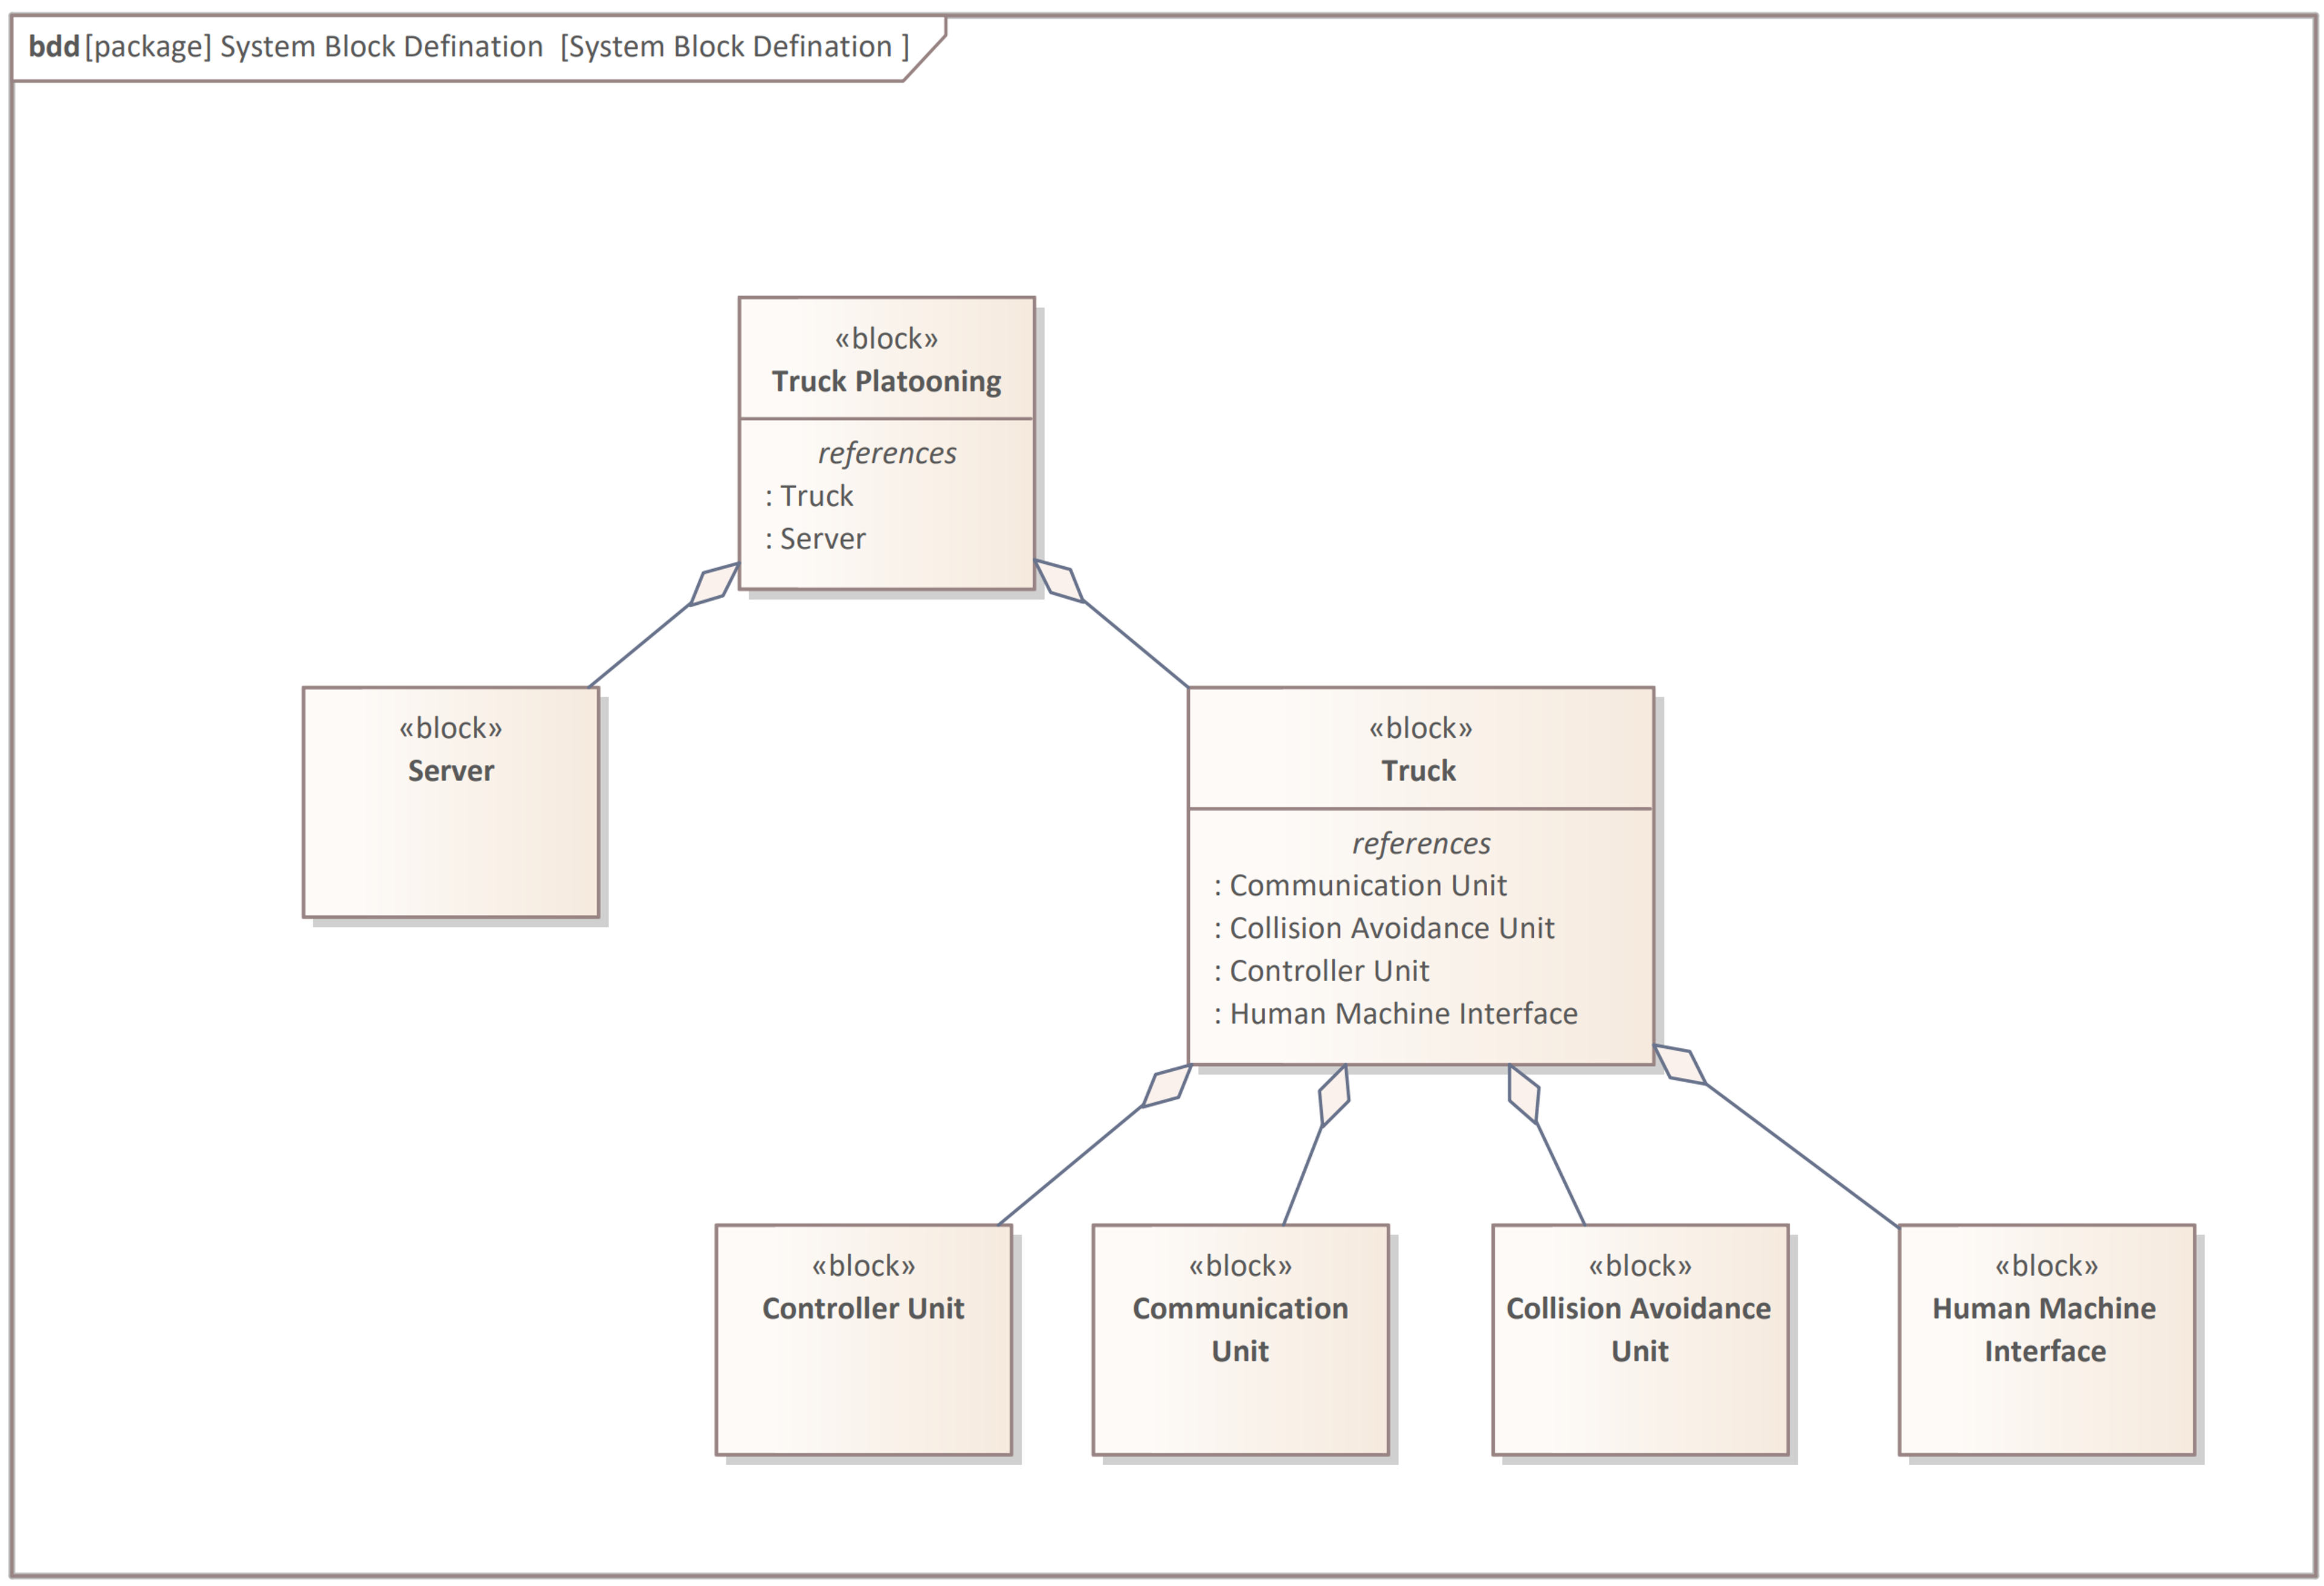
\includegraphics[width=0.5\textwidth]{images/system_bdd.png}
    \caption{System Architecture}
    \label{img:system_bdd}
\end{figure}